\section{Fragments}
In short a fragment in Android is functioning much like iFrames in HTML, meaning that a fragment is an embedded activity within another activity.
According to Google the design philosophy of fragments are that they support a more dynamic and versatile design of applications on devices with larger screens, such as tablets.
Google states that on these kind of devices there are more room to combine and interchange interface components, compared to a handset. 
An example of the use of multiple fragments on a large screen compared to activities on smaller handsets, is the Gmail application from Google:


\begin{figure}[H]
	\centering
		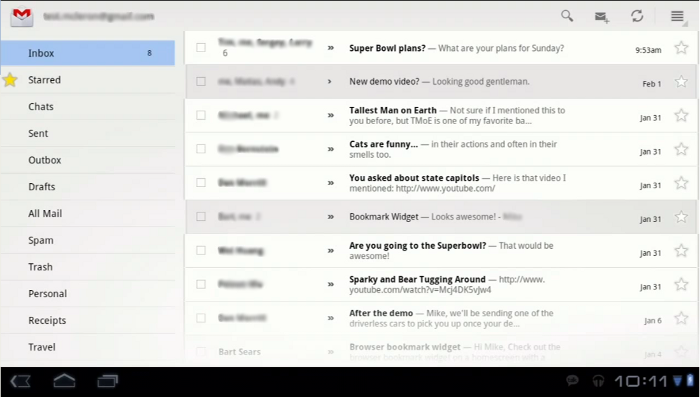
\includegraphics[width=\textwidt]{Images/Implementation/fragment_gmail.png}
			\caption{The Gmail application from Google on a tablet with fragment support.}
	\label{fig:fragment_gmail}
\end{figure}

\begin{figure}[H]
	\centering
		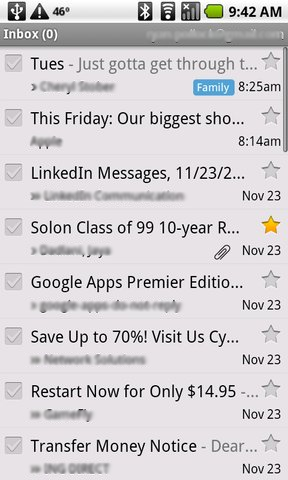
\includegraphics[scale=0.4]{Images/Implementation/fragment_gmail_handset.png}
	\caption{The Gmail application from Google on a handset without fragments}
	\label{fig:fragment_gmail_handset}
\end{figure}


This and more information about fragments can be found at \cite{web:android:fragments}.

\subsection{Benefits and Limitations}
%What is the benefits of a fragment compared to an activity
%Which Android versions support fragments
Fragments alone are not more powerful than activities and fragments can not exist without activities.
When combining multiple fragments in one activity, the fragments are able to create dynamic interfaces which does not require the entire activity to be reloaded when changing an object on the screen.\\

The Gmail application utilizes this by having an overview of the email account on the left side of the device while showing specific mail content on the right side as seen in figure \ref{fig:fragment_gmail}.

Fragments are built to be reused in multiple activities, which means that a single fragment can be used in several ways depending on the platform.
The main activity only has to declare which fragments it holds in the layout.

Fragments were introduced the first time with the Android 3.0 platform (API version 11). 
But as of 3rd March 2011 Google has made the "`Android Compatibility Package"', a library which let Android 1.6 devices or newer support fragments \cite{web:android:fragments:support}.
Mobile tuts+, a website about tutorials for Android development, has tested the "`Android Compatibility Package"' and they successfully used fragments with the support library on the T-Mobile G1 (the first Android device) \cite{web:android:fragments:compatibility}.
 
\subsection{Fragments in WOMBAT}
%How do we use fragments in the application?
%How does fragments affect the application?
In WOMBAT we use fragments to give the user the ability to quickly switch between multiple children and configuration templates, when developing with fragments we are able to let each part of the screen update independently based on actions in the fragments.
This means that we, much like the Gmail application, can keep an overview of all children and their personal configurations, while having a detailed configuration page open at the same time.
Thus avoid requiring the user to switch screen to load previous defined configurations.\\

Having developed WOMBAT with fragments means that it is possible to create a handset version with few modifications, since it only requires the "`Android Compatibility Package"' library and some new activities to handle the fragments on a smaller screen.